\documentclass[aspectratio=169,12pt]{beamer}
\usepackage{fontspec}
\usepackage{booktabs}
\usepackage{graphicx}
\usepackage{amsmath}
\usepackage{xcolor}
\usepackage{tikz}
\usetikzlibrary{positioning,arrows.meta}
\pdfstringdefDisableCommands{\def\translate#1{#1}}

\definecolor{blue}{HTML}{0072B2}
\definecolor{sky}{HTML}{56B4E9}
\definecolor{green}{HTML}{009E73}
\definecolor{orange}{HTML}{E69F00}
\definecolor{vermillion}{HTML}{D55E00}
\definecolor{purple}{HTML}{CC79A7}
\setbeamercolor{structure}{fg=blue}
\setbeamercolor{frametitle}{fg=black}
\setbeamercolor{title}{fg=black}
\setbeamercolor{alerted text}{fg=vermillion}
\setbeamertemplate{navigation symbols}{}
\setbeamertemplate{footline}{\hfill\usebeamerfont{footline}\insertframenumber/\inserttotalframenumber\hspace{4mm}\vspace{2mm}}
\setbeamertemplate{itemize item}{\color{blue}\small$\bullet$}
\setbeamersize{text margin left=7mm,text margin right=7mm}
\graphicspath{{../assets/figures/}}
% Generated by Source/reporting/build_analysis_tables.py
\expandafter\def\csname result@audit_final_seeds\endcsname{3}
\expandafter\def\csname result@audit_jobs\endcsname{1,251}
\expandafter\def\csname result@bonus_deployed_parameters\endcsname{2,841,858}
\expandafter\def\csname result@bonus_labels_saved_nsmc\endcsname{not estimable}
\expandafter\def\csname result@bonus_labels_saved_shopping\endcsname{not estimable}
\expandafter\def\csname result@bonus_labels_saved_steam\endcsname{not estimable}
\expandafter\def\csname result@bonus_projection_parameters\endcsname{24,768}
\expandafter\def\csname result@bonus_source_labels\endcsname{4,000}
\expandafter\def\csname result@dataset_nsmc_test_rows\endcsname{49,110}
\expandafter\def\csname result@dataset_nsmc_train_rows\endcsname{130,797}
\expandafter\def\csname result@dataset_nsmc_validation_rows\endcsname{14,534}
\expandafter\def\csname result@dataset_shopping_test_rows\endcsname{19,990}
\expandafter\def\csname result@dataset_shopping_train_rows\endcsname{159,918}
\expandafter\def\csname result@dataset_shopping_validation_rows\endcsname{19,990}
\expandafter\def\csname result@dataset_steam_test_rows\endcsname{9,979}
\expandafter\def\csname result@dataset_steam_train_rows\endcsname{79,828}
\expandafter\def\csname result@dataset_steam_validation_rows\endcsname{9,979}
\expandafter\def\csname result@full_nsmc_avg_mlp_macro_f1\endcsname{81.36 $\pm$ 0.03 (3)}
\expandafter\def\csname result@full_nsmc_gru_macro_f1\endcsname{81.80 $\pm$ 0.02 (3)}
\expandafter\def\csname result@full_nsmc_lstm_macro_f1\endcsname{81.64 $\pm$ 0.36 (3)}
\expandafter\def\csname result@full_nsmc_mamba_macro_f1\endcsname{80.72 $\pm$ 0.12 (3)}
\expandafter\def\csname result@full_nsmc_tfidf_lr_macro_f1\endcsname{80.07 $\pm$ 0.00 (3)}
\expandafter\def\csname result@full_nsmc_tfidf_rf_macro_f1\endcsname{75.39 $\pm$ 0.01 (3)}
\expandafter\def\csname result@full_nsmc_tfidf_svm_macro_f1\endcsname{80.04 $\pm$ 0.00 (3)}
\expandafter\def\csname result@full_nsmc_tfidf_xgb_macro_f1\endcsname{68.94 $\pm$ 0.03 (3)}
\expandafter\def\csname result@full_nsmc_transformer_macro_f1\endcsname{81.85 $\pm$ 0.02 (3)}
\expandafter\def\csname result@full_shopping_avg_mlp_macro_f1\endcsname{88.62 $\pm$ 0.19 (3)}
\expandafter\def\csname result@full_shopping_gru_macro_f1\endcsname{89.04 $\pm$ 0.21 (3)}
\expandafter\def\csname result@full_shopping_lstm_macro_f1\endcsname{88.97 $\pm$ 0.13 (3)}
\expandafter\def\csname result@full_shopping_mamba_macro_f1\endcsname{88.09 $\pm$ 0.08 (3)}
\expandafter\def\csname result@full_shopping_tfidf_lr_macro_f1\endcsname{88.34 $\pm$ 0.00 (3)}
\expandafter\def\csname result@full_shopping_tfidf_rf_macro_f1\endcsname{85.09 $\pm$ 0.02 (3)}
\expandafter\def\csname result@full_shopping_tfidf_svm_macro_f1\endcsname{88.30 $\pm$ 0.00 (3)}
\expandafter\def\csname result@full_shopping_tfidf_xgb_macro_f1\endcsname{80.37 $\pm$ 0.05 (3)}
\expandafter\def\csname result@full_shopping_transformer_macro_f1\endcsname{89.14 $\pm$ 0.11 (3)}
\expandafter\def\csname result@full_steam_avg_mlp_macro_f1\endcsname{76.39 $\pm$ 0.14 (3)}
\expandafter\def\csname result@full_steam_gru_macro_f1\endcsname{76.60 $\pm$ 0.42 (3)}
\expandafter\def\csname result@full_steam_lstm_macro_f1\endcsname{76.68 $\pm$ 0.44 (3)}
\expandafter\def\csname result@full_steam_mamba_macro_f1\endcsname{75.39 $\pm$ 0.14 (3)}
\expandafter\def\csname result@full_steam_tfidf_lr_macro_f1\endcsname{75.82 $\pm$ 0.00 (3)}
\expandafter\def\csname result@full_steam_tfidf_rf_macro_f1\endcsname{72.48 $\pm$ 0.04 (3)}
\expandafter\def\csname result@full_steam_tfidf_svm_macro_f1\endcsname{75.67 $\pm$ 0.00 (3)}
\expandafter\def\csname result@full_steam_tfidf_xgb_macro_f1\endcsname{68.21 $\pm$ 0.09 (3)}
\expandafter\def\csname result@full_steam_transformer_macro_f1\endcsname{76.64 $\pm$ 0.21 (3)}
\expandafter\def\csname result@part1_crossover_nsmc\endcsname{64,000}
\expandafter\def\csname result@part1_crossover_shopping\endcsname{not observed through 159,918}
\expandafter\def\csname result@part1_crossover_steam\endcsname{not observed through 79,828}
\expandafter\def\csname result@story_bonus_db_vs_pool_nsmc_200\endcsname{+0.77}
\expandafter\def\csname result@story_bonus_db_vs_pool_shopping_200\endcsname{+0.61}
\expandafter\def\csname result@story_bonus_db_vs_pool_steam_200\endcsname{+0.07}
\expandafter\def\csname result@story_bonus_pool_vs_target_nsmc_200\endcsname{+12.05}
\expandafter\def\csname result@story_bonus_pool_vs_target_shopping_200\endcsname{+5.19}
\expandafter\def\csname result@story_bonus_pool_vs_target_steam_200\endcsname{+13.54}
\expandafter\def\csname result@story_bonus_pool_vs_tfidf_nsmc_200\endcsname{+2.20}
\expandafter\def\csname result@story_bonus_pool_vs_tfidf_shopping_200\endcsname{-2.81}
\expandafter\def\csname result@story_bonus_pool_vs_tfidf_steam_200\endcsname{+2.21}
\expandafter\def\csname result@story_db_cost_ratio_nsmc\endcsname{1.27}
\expandafter\def\csname result@story_db_cost_ratio_shopping\endcsname{1.41}
\expandafter\def\csname result@story_db_cost_ratio_steam\endcsname{1.08}
\expandafter\def\csname result@story_db_separation_change_nsmc\endcsname{-0.007}
\expandafter\def\csname result@story_db_separation_change_shopping\endcsname{+0.008}
\expandafter\def\csname result@story_db_separation_change_steam\endcsname{-0.007}
\expandafter\def\csname result@story_fit_ratio_nsmc\endcsname{46.5}
\expandafter\def\csname result@story_fit_ratio_shopping\endcsname{48.7}
\expandafter\def\csname result@story_fit_ratio_steam\endcsname{27.7}
\expandafter\def\csname result@story_full_best_neural_nsmc\endcsname{81.85}
\expandafter\def\csname result@story_full_best_neural_shopping\endcsname{89.14}
\expandafter\def\csname result@story_full_best_neural_steam\endcsname{76.68}
\expandafter\def\csname result@story_full_best_tfidf_nsmc\endcsname{80.07}
\expandafter\def\csname result@story_full_best_tfidf_shopping\endcsname{88.34}
\expandafter\def\csname result@story_full_best_tfidf_steam\endcsname{75.82}
\expandafter\def\csname result@story_full_gap_nsmc\endcsname{1.77}
\expandafter\def\csname result@story_full_gap_shopping\endcsname{0.81}
\expandafter\def\csname result@story_full_gap_steam\endcsname{0.85}
\expandafter\def\csname result@table_bonus_diagnostics_nsmc_db_cdsupcon_retention\endcsname{+0.005}
\expandafter\def\csname result@table_bonus_diagnostics_nsmc_db_cdsupcon_separation\endcsname{0.088}
\expandafter\def\csname result@table_bonus_diagnostics_nsmc_pooled_ce_retention\endcsname{+0.000}
\expandafter\def\csname result@table_bonus_diagnostics_nsmc_pooled_ce_separation\endcsname{0.095}
\expandafter\def\csname result@table_bonus_diagnostics_nsmc_supcon_retention\endcsname{-0.000}
\expandafter\def\csname result@table_bonus_diagnostics_nsmc_supcon_separation\endcsname{0.094}
\expandafter\def\csname result@table_bonus_diagnostics_shopping_db_cdsupcon_retention\endcsname{+0.015}
\expandafter\def\csname result@table_bonus_diagnostics_shopping_db_cdsupcon_separation\endcsname{0.086}
\expandafter\def\csname result@table_bonus_diagnostics_shopping_pooled_ce_retention\endcsname{+0.000}
\expandafter\def\csname result@table_bonus_diagnostics_shopping_pooled_ce_separation\endcsname{0.078}
\expandafter\def\csname result@table_bonus_diagnostics_shopping_supcon_retention\endcsname{+0.015}
\expandafter\def\csname result@table_bonus_diagnostics_shopping_supcon_separation\endcsname{0.091}
\expandafter\def\csname result@table_bonus_diagnostics_steam_db_cdsupcon_retention\endcsname{-0.001}
\expandafter\def\csname result@table_bonus_diagnostics_steam_db_cdsupcon_separation\endcsname{0.147}
\expandafter\def\csname result@table_bonus_diagnostics_steam_pooled_ce_retention\endcsname{+0.000}
\expandafter\def\csname result@table_bonus_diagnostics_steam_pooled_ce_separation\endcsname{0.154}
\expandafter\def\csname result@table_bonus_diagnostics_steam_supcon_retention\endcsname{-0.001}
\expandafter\def\csname result@table_bonus_diagnostics_steam_supcon_separation\endcsname{0.146}
\expandafter\def\csname result@table_bonus_labels_nsmc_db_cdsupcon_crossover\endcsname{200}
\expandafter\def\csname result@table_bonus_labels_nsmc_db_cdsupcon_saved\endcsname{Not estimable}
\expandafter\def\csname result@table_bonus_labels_nsmc_pooled_ce_crossover\endcsname{200}
\expandafter\def\csname result@table_bonus_labels_nsmc_pooled_ce_saved\endcsname{Not estimable}
\expandafter\def\csname result@table_bonus_labels_nsmc_supcon_crossover\endcsname{200}
\expandafter\def\csname result@table_bonus_labels_nsmc_supcon_saved\endcsname{Not estimable}
\expandafter\def\csname result@table_bonus_labels_nsmc_target_transformer_crossover\endcsname{Not observed}
\expandafter\def\csname result@table_bonus_labels_nsmc_target_transformer_saved\endcsname{Not estimable}
\expandafter\def\csname result@table_bonus_labels_shopping_db_cdsupcon_crossover\endcsname{Not observed}
\expandafter\def\csname result@table_bonus_labels_shopping_db_cdsupcon_saved\endcsname{Not estimable}
\expandafter\def\csname result@table_bonus_labels_shopping_pooled_ce_crossover\endcsname{Not observed}
\expandafter\def\csname result@table_bonus_labels_shopping_pooled_ce_saved\endcsname{Not estimable}
\expandafter\def\csname result@table_bonus_labels_shopping_supcon_crossover\endcsname{Not observed}
\expandafter\def\csname result@table_bonus_labels_shopping_supcon_saved\endcsname{Not estimable}
\expandafter\def\csname result@table_bonus_labels_shopping_target_transformer_crossover\endcsname{Not observed}
\expandafter\def\csname result@table_bonus_labels_shopping_target_transformer_saved\endcsname{Not estimable}
\expandafter\def\csname result@table_bonus_labels_steam_db_cdsupcon_crossover\endcsname{200}
\expandafter\def\csname result@table_bonus_labels_steam_db_cdsupcon_saved\endcsname{Not estimable}
\expandafter\def\csname result@table_bonus_labels_steam_pooled_ce_crossover\endcsname{200}
\expandafter\def\csname result@table_bonus_labels_steam_pooled_ce_saved\endcsname{Not estimable}
\expandafter\def\csname result@table_bonus_labels_steam_supcon_crossover\endcsname{200}
\expandafter\def\csname result@table_bonus_labels_steam_supcon_saved\endcsname{Not estimable}
\expandafter\def\csname result@table_bonus_labels_steam_target_transformer_crossover\endcsname{Not observed}
\expandafter\def\csname result@table_bonus_labels_steam_target_transformer_saved\endcsname{Not estimable}
\expandafter\def\csname result@table_bonus_nsmc_best_tfidf_1000\endcsname{67.02 $\pm$ 0.28 (3)}
\expandafter\def\csname result@table_bonus_nsmc_best_tfidf_200\endcsname{60.62 $\pm$ 0.96 (3)}
\expandafter\def\csname result@table_bonus_nsmc_best_tfidf_2000\endcsname{69.65 $\pm$ 0.19 (3)}
\expandafter\def\csname result@table_bonus_nsmc_best_tfidf_500\endcsname{63.99 $\pm$ 0.58 (3)}
\expandafter\def\csname result@table_bonus_nsmc_db_cdsupcon_1000\endcsname{66.53 $\pm$ 0.74 (3)}
\expandafter\def\csname result@table_bonus_nsmc_db_cdsupcon_200\endcsname{63.59 $\pm$ 0.75 (3)}
\expandafter\def\csname result@table_bonus_nsmc_db_cdsupcon_2000\endcsname{68.78 $\pm$ 0.62 (3)}
\expandafter\def\csname result@table_bonus_nsmc_db_cdsupcon_500\endcsname{65.36 $\pm$ 0.34 (3)}
\expandafter\def\csname result@table_bonus_nsmc_pooled_ce_1000\endcsname{66.55 $\pm$ 1.07 (3)}
\expandafter\def\csname result@table_bonus_nsmc_pooled_ce_200\endcsname{62.82 $\pm$ 0.83 (3)}
\expandafter\def\csname result@table_bonus_nsmc_pooled_ce_2000\endcsname{68.71 $\pm$ 0.38 (3)}
\expandafter\def\csname result@table_bonus_nsmc_pooled_ce_500\endcsname{64.73 $\pm$ 1.33 (3)}
\expandafter\def\csname result@table_bonus_nsmc_supcon_1000\endcsname{66.02 $\pm$ 1.80 (3)}
\expandafter\def\csname result@table_bonus_nsmc_supcon_200\endcsname{63.08 $\pm$ 0.79 (3)}
\expandafter\def\csname result@table_bonus_nsmc_supcon_2000\endcsname{68.52 $\pm$ 0.68 (3)}
\expandafter\def\csname result@table_bonus_nsmc_supcon_500\endcsname{64.83 $\pm$ 1.32 (3)}
\expandafter\def\csname result@table_bonus_nsmc_target_transformer_1000\endcsname{54.72 $\pm$ 5.97 (3)}
\expandafter\def\csname result@table_bonus_nsmc_target_transformer_200\endcsname{50.77 $\pm$ 3.52 (3)}
\expandafter\def\csname result@table_bonus_nsmc_target_transformer_2000\endcsname{57.90 $\pm$ 1.17 (3)}
\expandafter\def\csname result@table_bonus_nsmc_target_transformer_500\endcsname{51.26 $\pm$ 6.13 (3)}
\expandafter\def\csname result@table_bonus_shopping_best_tfidf_1000\endcsname{79.81 $\pm$ 0.44 (3)}
\expandafter\def\csname result@table_bonus_shopping_best_tfidf_200\endcsname{71.93 $\pm$ 0.96 (3)}
\expandafter\def\csname result@table_bonus_shopping_best_tfidf_2000\endcsname{81.86 $\pm$ 0.31 (3)}
\expandafter\def\csname result@table_bonus_shopping_best_tfidf_500\endcsname{76.73 $\pm$ 1.52 (3)}
\expandafter\def\csname result@table_bonus_shopping_db_cdsupcon_1000\endcsname{75.35 $\pm$ 1.70 (3)}
\expandafter\def\csname result@table_bonus_shopping_db_cdsupcon_200\endcsname{69.73 $\pm$ 3.77 (3)}
\expandafter\def\csname result@table_bonus_shopping_db_cdsupcon_2000\endcsname{77.88 $\pm$ 0.69 (3)}
\expandafter\def\csname result@table_bonus_shopping_db_cdsupcon_500\endcsname{74.30 $\pm$ 0.46 (3)}
\expandafter\def\csname result@table_bonus_shopping_pooled_ce_1000\endcsname{75.86 $\pm$ 1.58 (3)}
\expandafter\def\csname result@table_bonus_shopping_pooled_ce_200\endcsname{69.11 $\pm$ 3.29 (3)}
\expandafter\def\csname result@table_bonus_shopping_pooled_ce_2000\endcsname{75.45 $\pm$ 2.19 (3)}
\expandafter\def\csname result@table_bonus_shopping_pooled_ce_500\endcsname{74.02 $\pm$ 0.67 (3)}
\expandafter\def\csname result@table_bonus_shopping_supcon_1000\endcsname{75.52 $\pm$ 1.70 (3)}
\expandafter\def\csname result@table_bonus_shopping_supcon_200\endcsname{69.48 $\pm$ 3.63 (3)}
\expandafter\def\csname result@table_bonus_shopping_supcon_2000\endcsname{78.04 $\pm$ 0.70 (3)}
\expandafter\def\csname result@table_bonus_shopping_supcon_500\endcsname{74.22 $\pm$ 0.85 (3)}
\expandafter\def\csname result@table_bonus_shopping_target_transformer_1000\endcsname{72.51 $\pm$ 2.31 (3)}
\expandafter\def\csname result@table_bonus_shopping_target_transformer_200\endcsname{63.92 $\pm$ 2.74 (3)}
\expandafter\def\csname result@table_bonus_shopping_target_transformer_2000\endcsname{71.75 $\pm$ 7.66 (3)}
\expandafter\def\csname result@table_bonus_shopping_target_transformer_500\endcsname{64.70 $\pm$ 5.53 (3)}
\expandafter\def\csname result@table_bonus_steam_best_tfidf_1000\endcsname{64.49 $\pm$ 0.46 (3)}
\expandafter\def\csname result@table_bonus_steam_best_tfidf_200\endcsname{60.50 $\pm$ 0.60 (3)}
\expandafter\def\csname result@table_bonus_steam_best_tfidf_2000\endcsname{67.32 $\pm$ 0.44 (3)}
\expandafter\def\csname result@table_bonus_steam_best_tfidf_500\endcsname{62.42 $\pm$ 0.58 (3)}
\expandafter\def\csname result@table_bonus_steam_db_cdsupcon_1000\endcsname{64.97 $\pm$ 0.84 (3)}
\expandafter\def\csname result@table_bonus_steam_db_cdsupcon_200\endcsname{62.78 $\pm$ 1.50 (3)}
\expandafter\def\csname result@table_bonus_steam_db_cdsupcon_2000\endcsname{66.14 $\pm$ 0.66 (3)}
\expandafter\def\csname result@table_bonus_steam_db_cdsupcon_500\endcsname{62.83 $\pm$ 0.92 (3)}
\expandafter\def\csname result@table_bonus_steam_pooled_ce_1000\endcsname{65.18 $\pm$ 0.35 (3)}
\expandafter\def\csname result@table_bonus_steam_pooled_ce_200\endcsname{62.71 $\pm$ 1.04 (3)}
\expandafter\def\csname result@table_bonus_steam_pooled_ce_2000\endcsname{66.29 $\pm$ 0.41 (3)}
\expandafter\def\csname result@table_bonus_steam_pooled_ce_500\endcsname{62.83 $\pm$ 1.33 (3)}
\expandafter\def\csname result@table_bonus_steam_supcon_1000\endcsname{64.67 $\pm$ 0.57 (3)}
\expandafter\def\csname result@table_bonus_steam_supcon_200\endcsname{61.70 $\pm$ 0.20 (3)}
\expandafter\def\csname result@table_bonus_steam_supcon_2000\endcsname{66.51 $\pm$ 0.97 (3)}
\expandafter\def\csname result@table_bonus_steam_supcon_500\endcsname{63.93 $\pm$ 0.14 (3)}
\expandafter\def\csname result@table_bonus_steam_target_transformer_1000\endcsname{58.02 $\pm$ 1.87 (3)}
\expandafter\def\csname result@table_bonus_steam_target_transformer_200\endcsname{49.18 $\pm$ 2.60 (3)}
\expandafter\def\csname result@table_bonus_steam_target_transformer_2000\endcsname{57.33 $\pm$ 5.48 (3)}
\expandafter\def\csname result@table_bonus_steam_target_transformer_500\endcsname{54.20 $\pm$ 1.14 (3)}
\expandafter\def\csname result@table_completeness_bonus_final\endcsname{108}
\expandafter\def\csname result@table_completeness_bonus_tuning\endcsname{36}
\expandafter\def\csname result@table_completeness_part1_final\endcsname{837}
\expandafter\def\csname result@table_completeness_part1_tuning\endcsname{270}
\expandafter\def\csname result@table_completeness_total\endcsname{1,251}
\expandafter\def\csname result@table_config_nsmc_avg_mlp\endcsname{mlp08: {"dropout": 0.3, "embedding_dim": 128, "hidden_dim": 288, "id": "mlp08", "learning_rate": 0.002, "num_layers": 2}}
\expandafter\def\csname result@table_config_nsmc_gru\endcsname{gru08: {"dropout": 0.3, "embedding_dim": 128, "hidden_dim": 128, "id": "gru08", "learning_rate": 0.002, "num_layers": 2}}
\expandafter\def\csname result@table_config_nsmc_lstm\endcsname{lstm08: {"dropout": 0.3, "embedding_dim": 128, "hidden_dim": 112, "id": "lstm08", "learning_rate": 0.002, "num_layers": 2}}
\expandafter\def\csname result@table_config_nsmc_mamba\endcsname{mb08: {"d_conv": 4, "d_state": 16, "dropout": 0.3, "embedding_dim": 128, "expand": 2, "hidden_dim": 128, "id": "mb08", "learning_rate": 0.002, "num_layers": 2}}
\expandafter\def\csname result@table_config_nsmc_tfidf_lr\endcsname{lr06: {"C": 2.0, "id": "lr06", "max_iter": 3000, "solver": "liblinear"}}
\expandafter\def\csname result@table_config_nsmc_tfidf_rf\endcsname{rf09: {"id": "rf09", "max_depth": null, "max_features": "sqrt", "min_samples_leaf": 2, "n_estimators": 700}}
\expandafter\def\csname result@table_config_nsmc_tfidf_svm\endcsname{svm05: {"C": 0.25, "id": "svm05"}}
\expandafter\def\csname result@table_config_nsmc_tfidf_xgb\endcsname{xgb03: {"colsample_bytree": 0.8, "id": "xgb03", "learning_rate": 0.05, "max_depth": 4, "n_estimators": 400, "reg_lambda": 1.0, "subsample": 0.8}}
\expandafter\def\csname result@table_config_nsmc_transformer\endcsname{tr07: {"dropout": 0.4, "embedding_dim": 128, "ff_multiplier": 2, "hidden_dim": 128, "id": "tr07", "learning_rate": 0.001, "num_heads": 4, "num_layers": 2}}
\expandafter\def\csname result@table_config_shopping_avg_mlp\endcsname{mlp08: {"dropout": 0.3, "embedding_dim": 128, "hidden_dim": 288, "id": "mlp08", "learning_rate": 0.002, "num_layers": 2}}
\expandafter\def\csname result@table_config_shopping_gru\endcsname{gru08: {"dropout": 0.3, "embedding_dim": 128, "hidden_dim": 128, "id": "gru08", "learning_rate": 0.002, "num_layers": 2}}
\expandafter\def\csname result@table_config_shopping_lstm\endcsname{lstm04: {"dropout": 0.2, "embedding_dim": 96, "hidden_dim": 96, "id": "lstm04", "learning_rate": 0.002, "num_layers": 1}}
\expandafter\def\csname result@table_config_shopping_mamba\endcsname{mb08: {"d_conv": 4, "d_state": 16, "dropout": 0.3, "embedding_dim": 128, "expand": 2, "hidden_dim": 128, "id": "mb08", "learning_rate": 0.002, "num_layers": 2}}
\expandafter\def\csname result@table_config_shopping_tfidf_lr\endcsname{lr06: {"C": 2.0, "id": "lr06", "max_iter": 3000, "solver": "liblinear"}}
\expandafter\def\csname result@table_config_shopping_tfidf_rf\endcsname{rf09: {"id": "rf09", "max_depth": null, "max_features": "sqrt", "min_samples_leaf": 2, "n_estimators": 700}}
\expandafter\def\csname result@table_config_shopping_tfidf_svm\endcsname{svm05: {"C": 0.25, "id": "svm05"}}
\expandafter\def\csname result@table_config_shopping_tfidf_xgb\endcsname{xgb03: {"colsample_bytree": 0.8, "id": "xgb03", "learning_rate": 0.05, "max_depth": 4, "n_estimators": 400, "reg_lambda": 1.0, "subsample": 0.8}}
\expandafter\def\csname result@table_config_shopping_transformer\endcsname{tr07: {"dropout": 0.4, "embedding_dim": 128, "ff_multiplier": 2, "hidden_dim": 128, "id": "tr07", "learning_rate": 0.001, "num_heads": 4, "num_layers": 2}}
\expandafter\def\csname result@table_config_steam_avg_mlp\endcsname{mlp08: {"dropout": 0.3, "embedding_dim": 128, "hidden_dim": 288, "id": "mlp08", "learning_rate": 0.002, "num_layers": 2}}
\expandafter\def\csname result@table_config_steam_gru\endcsname{gru08: {"dropout": 0.3, "embedding_dim": 128, "hidden_dim": 128, "id": "gru08", "learning_rate": 0.002, "num_layers": 2}}
\expandafter\def\csname result@table_config_steam_lstm\endcsname{lstm08: {"dropout": 0.3, "embedding_dim": 128, "hidden_dim": 112, "id": "lstm08", "learning_rate": 0.002, "num_layers": 2}}
\expandafter\def\csname result@table_config_steam_mamba\endcsname{mb07: {"d_conv": 3, "d_state": 16, "dropout": 0.4, "embedding_dim": 128, "expand": 2, "hidden_dim": 128, "id": "mb07", "learning_rate": 0.001, "num_layers": 2}}
\expandafter\def\csname result@table_config_steam_tfidf_lr\endcsname{lr06: {"C": 2.0, "id": "lr06", "max_iter": 3000, "solver": "liblinear"}}
\expandafter\def\csname result@table_config_steam_tfidf_rf\endcsname{rf09: {"id": "rf09", "max_depth": null, "max_features": "sqrt", "min_samples_leaf": 2, "n_estimators": 700}}
\expandafter\def\csname result@table_config_steam_tfidf_svm\endcsname{svm05: {"C": 0.25, "id": "svm05"}}
\expandafter\def\csname result@table_config_steam_tfidf_xgb\endcsname{xgb03: {"colsample_bytree": 0.8, "id": "xgb03", "learning_rate": 0.05, "max_depth": 4, "n_estimators": 400, "reg_lambda": 1.0, "subsample": 0.8}}
\expandafter\def\csname result@table_config_steam_transformer\endcsname{tr08: {"dropout": 0.3, "embedding_dim": 128, "ff_multiplier": 2, "hidden_dim": 128, "id": "tr08", "learning_rate": 0.002, "num_heads": 8, "num_layers": 2}}
\expandafter\def\csname result@table_crossover_nsmc_observed\endcsname{64,000}
\expandafter\def\csname result@table_crossover_nsmc_sustained\endcsname{64,000}
\expandafter\def\csname result@table_crossover_shopping_observed\endcsname{Not through 159,918}
\expandafter\def\csname result@table_crossover_shopping_sustained\endcsname{Not through 159,918}
\expandafter\def\csname result@table_crossover_steam_observed\endcsname{Not through 79,828}
\expandafter\def\csname result@table_crossover_steam_sustained\endcsname{Not through 79,828}
\expandafter\def\csname result@table_dataset_nsmc_n_full\endcsname{130,797}
\expandafter\def\csname result@table_dataset_nsmc_test_positive_pct\endcsname{50.3}
\expandafter\def\csname result@table_dataset_nsmc_test_rows\endcsname{49,110}
\expandafter\def\csname result@table_dataset_nsmc_train_positive_pct\endcsname{49.8}
\expandafter\def\csname result@table_dataset_nsmc_train_rows\endcsname{130,797}
\expandafter\def\csname result@table_dataset_nsmc_validation_positive_pct\endcsname{49.8}
\expandafter\def\csname result@table_dataset_nsmc_validation_rows\endcsname{14,534}
\expandafter\def\csname result@table_dataset_shopping_n_full\endcsname{159,918}
\expandafter\def\csname result@table_dataset_shopping_test_positive_pct\endcsname{50.0}
\expandafter\def\csname result@table_dataset_shopping_test_rows\endcsname{19,990}
\expandafter\def\csname result@table_dataset_shopping_train_positive_pct\endcsname{50.0}
\expandafter\def\csname result@table_dataset_shopping_train_rows\endcsname{159,918}
\expandafter\def\csname result@table_dataset_shopping_validation_positive_pct\endcsname{50.0}
\expandafter\def\csname result@table_dataset_shopping_validation_rows\endcsname{19,990}
\expandafter\def\csname result@table_dataset_steam_n_full\endcsname{79,828}
\expandafter\def\csname result@table_dataset_steam_test_positive_pct\endcsname{50.0}
\expandafter\def\csname result@table_dataset_steam_test_rows\endcsname{9,979}
\expandafter\def\csname result@table_dataset_steam_train_positive_pct\endcsname{50.0}
\expandafter\def\csname result@table_dataset_steam_train_rows\endcsname{79,828}
\expandafter\def\csname result@table_dataset_steam_validation_positive_pct\endcsname{50.0}
\expandafter\def\csname result@table_dataset_steam_validation_rows\endcsname{9,979}
\expandafter\def\csname result@table_efficiency_nsmc_tfidf_lr_fit_time\endcsname{5.1}
\expandafter\def\csname result@table_efficiency_nsmc_tfidf_lr_latency\endcsname{0.50}
\expandafter\def\csname result@table_efficiency_nsmc_tfidf_lr_macro_f1\endcsname{80.07}
\expandafter\def\csname result@table_efficiency_nsmc_tfidf_lr_peak_memory\endcsname{1702}
\expandafter\def\csname result@table_efficiency_nsmc_tfidf_lr_size\endcsname{0.42}
\expandafter\def\csname result@table_efficiency_nsmc_transformer_fit_time\endcsname{235.9}
\expandafter\def\csname result@table_efficiency_nsmc_transformer_latency\endcsname{1.87}
\expandafter\def\csname result@table_efficiency_nsmc_transformer_macro_f1\endcsname{81.85}
\expandafter\def\csname result@table_efficiency_nsmc_transformer_peak_memory\endcsname{335}
\expandafter\def\csname result@table_efficiency_nsmc_transformer_size\endcsname{11.23}
\expandafter\def\csname result@table_efficiency_shopping_tfidf_lr_fit_time\endcsname{5.9}
\expandafter\def\csname result@table_efficiency_shopping_tfidf_lr_latency\endcsname{0.50}
\expandafter\def\csname result@table_efficiency_shopping_tfidf_lr_macro_f1\endcsname{88.34}
\expandafter\def\csname result@table_efficiency_shopping_tfidf_lr_peak_memory\endcsname{3483}
\expandafter\def\csname result@table_efficiency_shopping_tfidf_lr_size\endcsname{0.43}
\expandafter\def\csname result@table_efficiency_shopping_transformer_fit_time\endcsname{289.7}
\expandafter\def\csname result@table_efficiency_shopping_transformer_latency\endcsname{1.96}
\expandafter\def\csname result@table_efficiency_shopping_transformer_macro_f1\endcsname{89.14}
\expandafter\def\csname result@table_efficiency_shopping_transformer_peak_memory\endcsname{333}
\expandafter\def\csname result@table_efficiency_shopping_transformer_size\endcsname{11.24}
\expandafter\def\csname result@table_efficiency_steam_lstm_fit_time\endcsname{95.1}
\expandafter\def\csname result@table_efficiency_steam_lstm_latency\endcsname{1.03}
\expandafter\def\csname result@table_efficiency_steam_lstm_macro_f1\endcsname{76.68}
\expandafter\def\csname result@table_efficiency_steam_lstm_peak_memory\endcsname{176}
\expandafter\def\csname result@table_efficiency_steam_lstm_size\endcsname{12.13}
\expandafter\def\csname result@table_efficiency_steam_tfidf_lr_fit_time\endcsname{3.4}
\expandafter\def\csname result@table_efficiency_steam_tfidf_lr_latency\endcsname{0.52}
\expandafter\def\csname result@table_efficiency_steam_tfidf_lr_macro_f1\endcsname{75.82}
\expandafter\def\csname result@table_efficiency_steam_tfidf_lr_peak_memory\endcsname{2162}
\expandafter\def\csname result@table_efficiency_steam_tfidf_lr_size\endcsname{0.42}

\newcommand{\Result}[1]{\csname result@#1\endcsname}
\newcommand{\takeaway}[1]{\vfill\begin{beamercolorbox}[sep=5pt,wd=\linewidth]{block body}\normalsize\textbf{Takeaway:} #1\end{beamercolorbox}}

\title{How Much Labeled Data Do Korean Sentiment Models Need?}
\subtitle{A multi-domain scale benchmark with a cross-domain contrastive extension}
\author{Practical Machine Learning Course Project}
\date{November 2026}

\begin{document}

\begin{frame}[plain]
  \titlepage
  \vspace{-3mm}
  \centering
  \large Model choice changes with label scale, and the crossover is domain-dependent.
\end{frame}

\begin{frame}{Why measure the whole learning curve?}
  \begin{columns}[T]
    \column{0.48\textwidth}
    \Large\color{blue}200 labels
    \vspace{2mm}
    \begin{itemize}
      \item Sparse lexical evidence is easy to estimate
      \item Neural embeddings are mostly unlearned
      \item Training cost matters immediately
    \end{itemize}
    \column{0.48\textwidth}
    \Large\color{purple}Full cleaned pool
    \vspace{2mm}
    \begin{itemize}
      \item Sequence models can learn reusable patterns
      \item Small quality gaps may affect many predictions
      \item Deployment cost becomes the trade-off
    \end{itemize}
  \end{columns}
  \takeaway{A full-data leaderboard cannot tell us when a model becomes worthwhile.}
\end{frame}

\begin{frame}{Approved benchmark first; bonus transfer study second}
  \begin{columns}[T]
    \column{0.49\textwidth}
    \textbf{\color{blue}Part 1: approved main study}
    \begin{itemize}
      \item Three Korean review datasets
      \item Nine complete pipelines
      \item 200 labels to each full cleaned pool
      \item Performance crossover plus cost
    \end{itemize}
    \column{0.49\textwidth}
    \textbf{\color{purple}Part 2: bonus extension}
    \begin{itemize}
      \item One low-label target at a time
      \item Two source domains already labeled
      \item Pooled CE, SupCon, DB-CDSupCon
      \item Label efficiency and source retention
    \end{itemize}
  \end{columns}
  \takeaway{Continual learning and pretrained language models are outside the completed design.}
\end{frame}

\begin{frame}{Three domains, fixed splits, nested subsets}
  \centering
  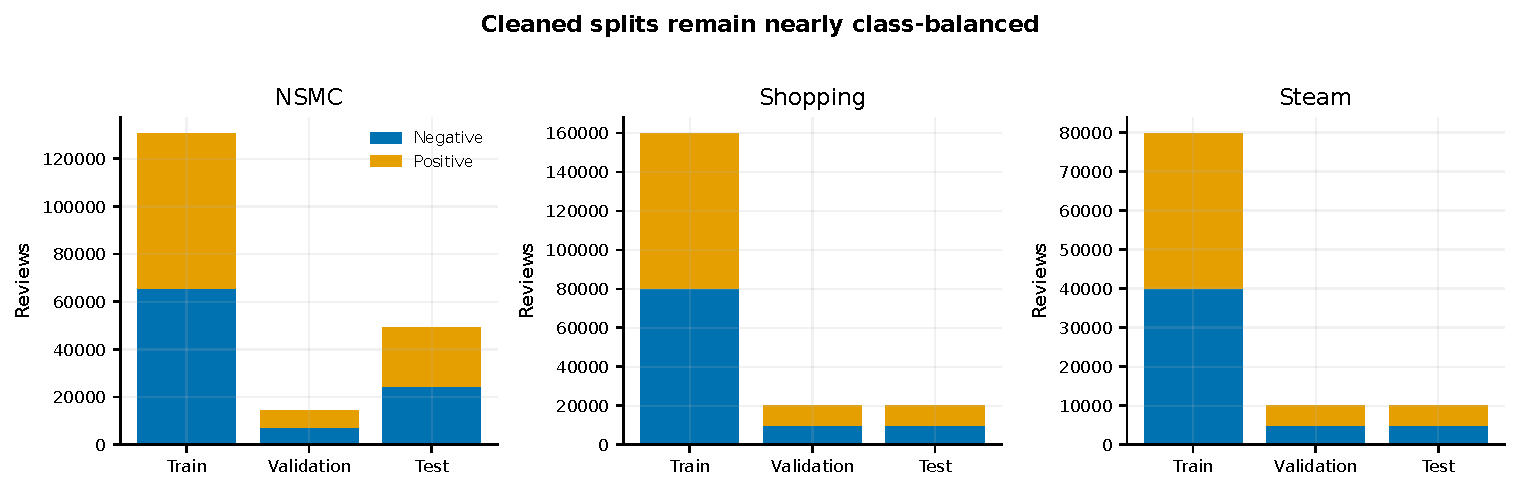
\includegraphics[width=0.88\textwidth]{dataset_overview.pdf}
  \takeaway{Every model sees the same example IDs for a dataset, size, and seed.}
\end{frame}

\begin{frame}{Nine Part 1 pipelines under one protocol}
  \begin{columns}[T]
    \column{0.47\textwidth}
    \textbf{\color{blue}TF-IDF family}
    \begin{itemize}
      \item Logistic regression
      \item Linear SVM
      \item Random Forest
      \item XGBoost
    \end{itemize}
    \column{0.47\textwidth}
    \textbf{\color{purple}Learned from scratch}
    \begin{itemize}
      \item Average embeddings + MLP
      \item LSTM and GRU
      \item Small Transformer
      \item Small Mamba
    \end{itemize}
  \end{columns}
  \vspace{4mm}
  \centering
  \small Same nested subsets $\cdot$ ten tuning candidates each $\cdot$ tuning at 8,000 $\cdot$ frozen configurations $\cdot$ final seeds 13, 42, 2026
  \takeaway{Fairness comes from shared data and selection rules, not matched representations.}
\end{frame}

\begin{frame}{Primary metric and crossover definition}
  \begin{columns}[c]
    \column{0.43\textwidth}
    \centering
    \Large Macro-F1
    \[
      \frac{F1_{\mathrm{negative}}+F1_{\mathrm{positive}}}{2}
    \]
    \column{0.54\textwidth}
    \Large First sustained crossover
    \[
      \bar F_{1,\mathrm{neural}}(n)-\bar F_{1,\mathrm{TFIDF}}(n)\geq 0.01
    \]
    \normalsize at size $n$ \textbf{and every larger tested size}
  \end{columns}
  \vspace{3mm}
  \centering
  Means and sample SD use three final seeds. No formal significance claim.
  \takeaway{The threshold is prespecified and sustained, so one isolated win is insufficient.}
\end{frame}

\begin{frame}{Part 1: rankings change with label scale}
  \centering
  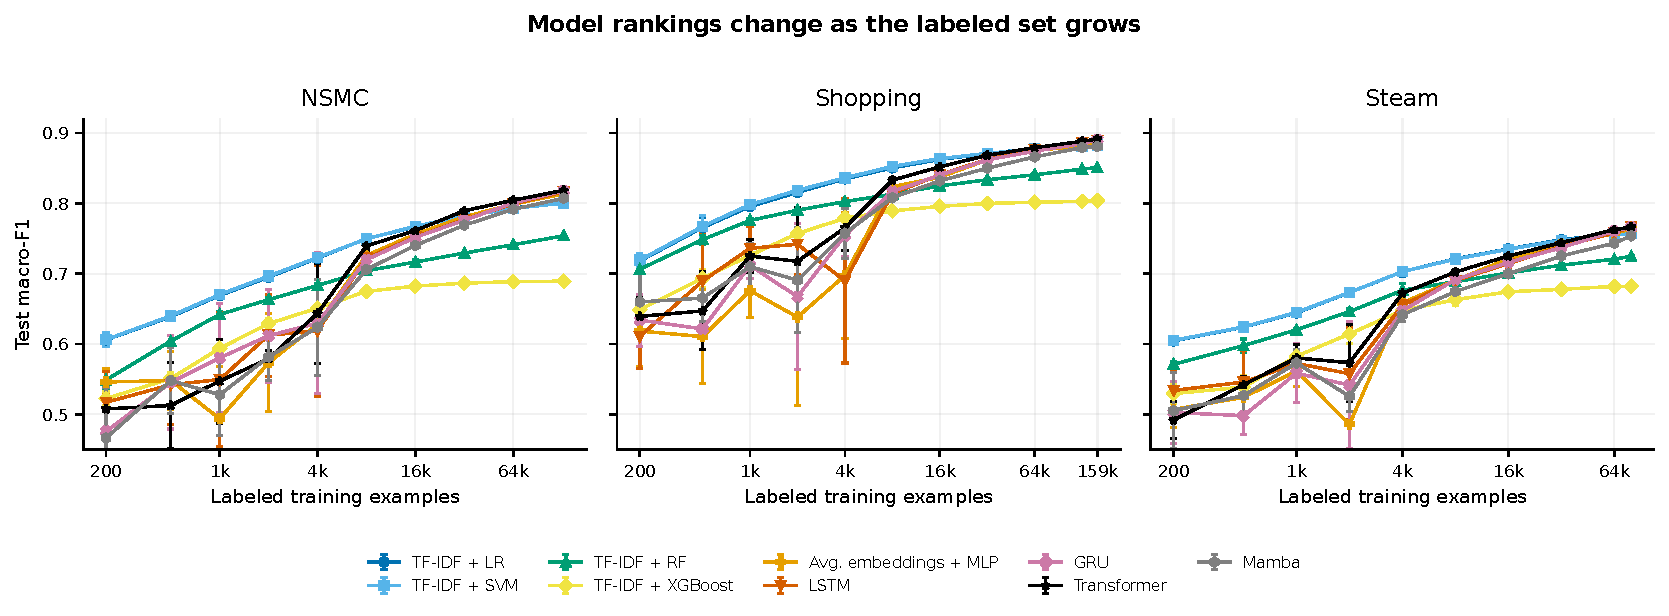
\includegraphics[width=0.96\textwidth]{part1_learning_curves.pdf}
  \takeaway{TF-IDF leads early; neural curves close the gap near the largest budgets.}
\end{frame}

\begin{frame}{Only NSMC reaches a sustained one-point crossover}
  \centering
  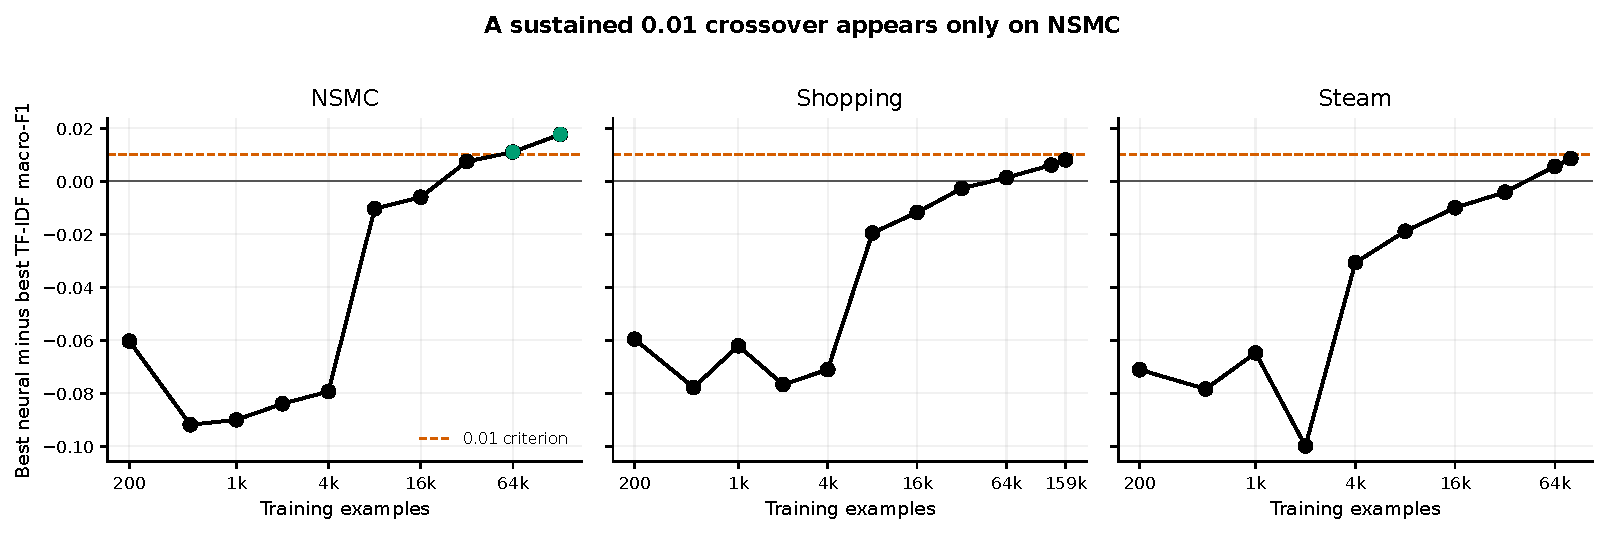
\includegraphics[width=0.88\textwidth]{part1_crossover.pdf}
  \vspace{-1mm}
  \begin{columns}[T]
    \column{0.31\textwidth}\centering NSMC\\\textbf{\Result{part1_crossover_nsmc}}
    \column{0.34\textwidth}\centering Shopping\\{\small\textbf{\Result{part1_crossover_shopping}}}
    \column{0.31\textwidth}\centering Steam\\{\small\textbf{\Result{part1_crossover_steam}}}
  \end{columns}
  \takeaway{Neural models win at full data, but the prespecified margin is not universal.}
\end{frame}

\begin{frame}{The last fraction of macro-F1 is expensive}
  \centering
  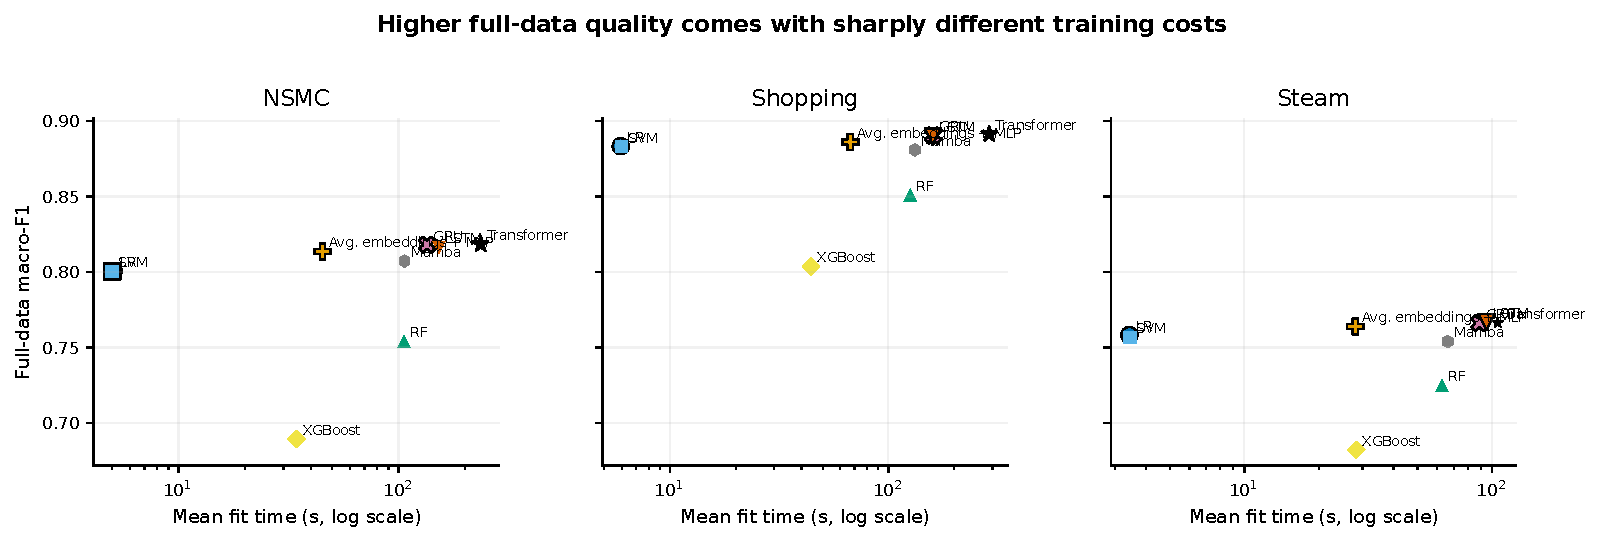
\includegraphics[width=0.88\textwidth]{efficiency_pareto.pdf}
  \vspace{-1mm}
  \small Best-neural fit-time ratios versus best TF-IDF:
  NSMC \Result{story_fit_ratio_nsmc}$\times$,
  Shopping \Result{story_fit_ratio_shopping}$\times$,
  Steam \Result{story_fit_ratio_steam}$\times$.
  \takeaway{Linear TF-IDF remains the practical default unless the final quality increment is valuable.}
\end{frame}

\begin{frame}{Why test cross-domain learning?}
  \begin{columns}[c]
    \column{0.45\textwidth}
      \centering
      \Large New target labels\\[2mm]
      \textbf{200, 500, 1,000, 2,000}
    \column{0.08\textwidth}
      \centering\Huge+
    \column{0.45\textwidth}
      \centering
      \Large Existing source labels\\[2mm]
      \textbf{2,000 + 2,000}
  \end{columns}
  \vspace{6mm}
  \begin{itemize}
    \item Rotate NSMC, Shopping, and Steam as the target
    \item Reuse Part 1 TF-IDF and target-only Transformer results
    \item Train only the three pooled objectives
  \end{itemize}
  \takeaway{The question is new target labels saved when source labels already exist, not total annotation savings.}
\end{frame}

\begin{frame}{Five methods separate pooling from the loss function}
  \begin{enumerate}
    \item Best Part 1 TF-IDF at the same target size
    \item Part 1 target-only Transformer + CE
    \item Pooled multi-domain Transformer + CE
    \item Pooled Transformer + standard SupCon
    \item Pooled Transformer + \textbf{DB-CDSupCon}
  \end{enumerate}
  \vspace{3mm}
  \centering
  \small Methods 1--2 reuse Part 1. Methods 3--5 share examples, backbone, sampler, seed, and optimizer.
  \takeaway{Pooled CE is the required baseline for attributing any gain to contrastive learning.}
\end{frame}

\begin{frame}{DB-CDSupCon emphasizes cross-domain positives}
  \centering
  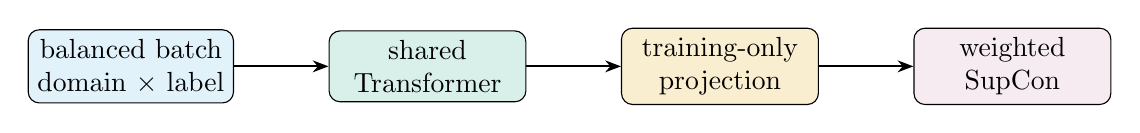
\begin{tikzpicture}[
    box/.style={draw,rounded corners,minimum width=2.5cm,minimum height=0.9cm,align=center},
    arrow/.style={-{Stealth[length=2mm]},thick}
  ]
    \node[box,fill=sky!18] (batch) {balanced batch\\domain $\times$ label};
    \node[box,fill=green!15,right=1.2cm of batch] (encoder) {shared\\Transformer};
    \node[box,fill=orange!18,right=1.2cm of encoder] (proj) {training-only\\projection};
    \node[box,fill=purple!15,right=1.2cm of proj] (loss) {weighted\\SupCon};
    \draw[arrow] (batch) -- (encoder);
    \draw[arrow] (encoder) -- (proj);
    \draw[arrow] (proj) -- (loss);
  \end{tikzpicture}
  \vspace{5mm}
  \[
    \tilde w_{ip}=
    \begin{cases}
      \alpha,&y_i=y_p,\ d_i\neq d_p\\
      1,&y_i=y_p,\ d_i=d_p
    \end{cases}
    \qquad
    \mathcal L=\mathcal L_{\mathrm{CE}}+\lambda\mathcal L_{\mathrm{SC}}
  \]
  \scriptsize SupCon: Khosla et al., NeurIPS 2020.
  \takeaway{Cross-domain same-sentiment pairs get more weight; deployment discards the projection head.}
\end{frame}

\begin{frame}{Pooling helps target-only CE; contrastive gains are mixed}
  \centering
  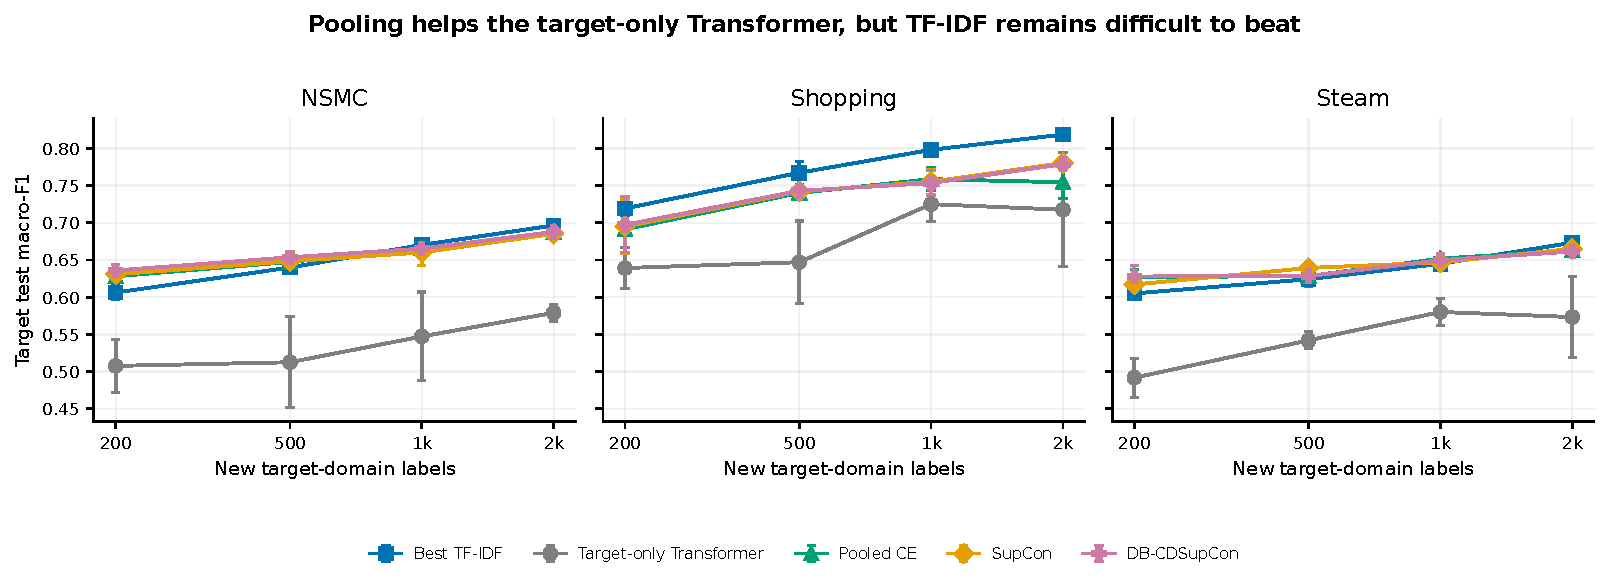
\includegraphics[width=0.94\textwidth]{bonus_learning_curves.pdf}
  \takeaway{The source-data effect is large, while SupCon and DB-CDSupCon change sign across cells.}
\end{frame}

\begin{frame}{The tested grid does not support a labels-saved number}
  \centering
  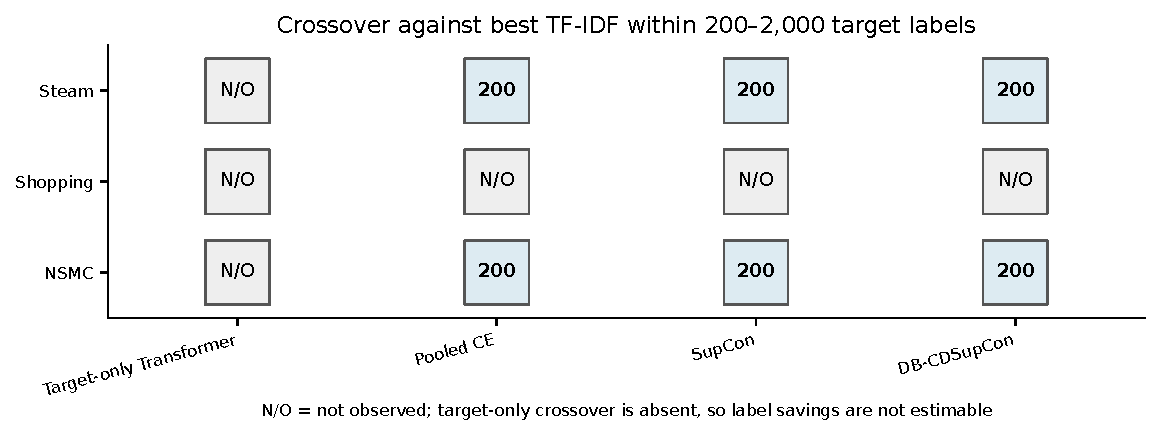
\includegraphics[width=0.72\textwidth]{bonus_crossover_status.pdf}
  \par\vspace{-1mm}
  {\small Target-only Transformer never reaches the TF-IDF + 0.01 threshold.\par}
  \takeaway{Without an observed target-only threshold, crossover shift and new target-label savings are not estimable.}
\end{frame}

\begin{frame}{Transfer, separation, and overhead do not move together}
  \begin{columns}[T]
    \column{0.58\textwidth}
      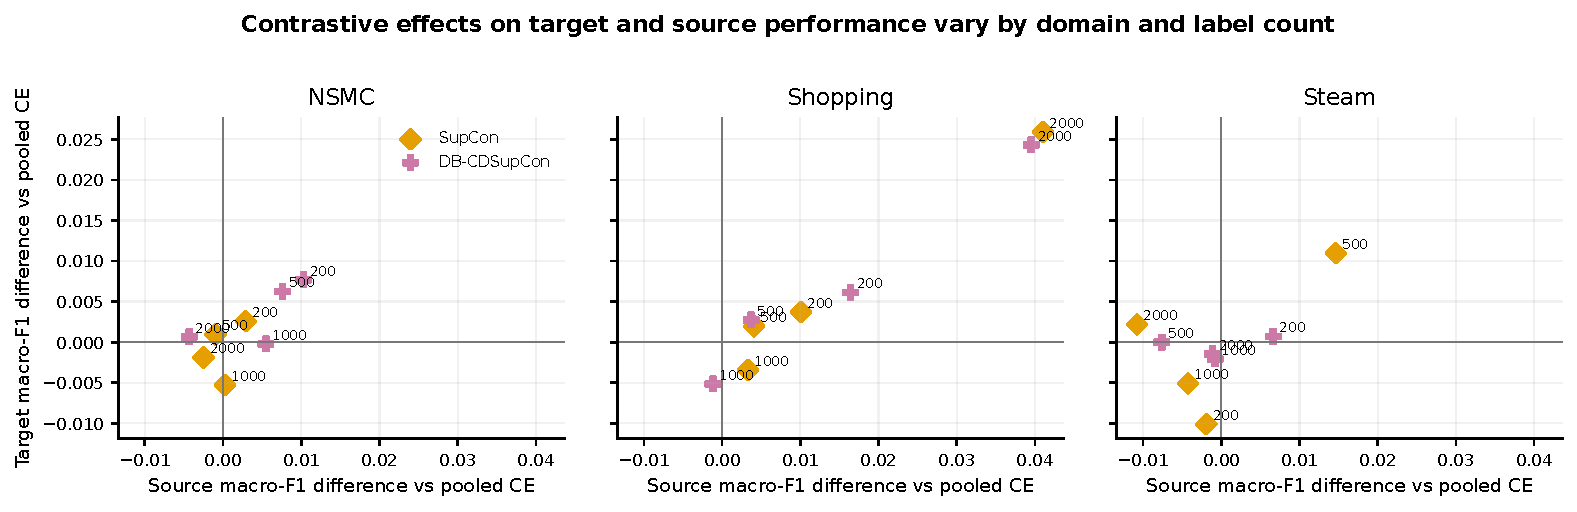
\includegraphics[width=\textwidth]{bonus_transfer.pdf}
    \column{0.4\textwidth}
      \begin{itemize}
        \item Source retention changes sign
        \item Separation improves only for Shopping on average
        \item DB fit-time ratio: \Result{story_db_cost_ratio_nsmc}$\times$ to \Result{story_db_cost_ratio_shopping}$\times$
        \item Same deployed \Result{bonus_deployed_parameters}-parameter classifier
      \end{itemize}
  \end{columns}
  \takeaway{A cleaner representation metric is not enough; target and source task metrics must agree.}
\end{frame}

\begin{frame}{What worked, what did not, and what is limited}
  \begin{columns}[T]
    \column{0.32\textwidth}
    \textbf{\color{green}Worked}
    \begin{itemize}
      \item Shared nested benchmark
      \item Clear NSMC crossover
      \item Pooling source labels
    \end{itemize}
    \column{0.32\textwidth}
    \textbf{\color{vermillion}Did not generalize}
    \begin{itemize}
      \item One crossover rule for all domains
      \item SupCon over pooled CE
      \item DB-CDSupCon dominance
    \end{itemize}
    \column{0.32\textwidth}
    \textbf{Limits}
    \begin{itemize}
      \item Three seeds
      \item No pretrained model
      \item Three binary domains
      \item Mixed CPU/GPU timing
    \end{itemize}
  \end{columns}
  \takeaway{The negative and mixed results narrow the conditions under which complexity is useful.}
\end{frame}

\begin{frame}{Four takeaways}
  \begin{enumerate}
    \item \textbf{Start with linear TF-IDF} at low and medium label budgets.
    \item \textbf{Expect domain-specific crossover:} only NSMC sustains the one-point neural margin.
    \item \textbf{Price the last quality increment:} the best neural fit takes \Result{story_fit_ratio_steam}$\times$--\Result{story_fit_ratio_shopping}$\times$ as long.
    \item \textbf{Pool before adding contrastive losses:} source labels help, but SupCon variants do not dominate pooled CE.
  \end{enumerate}
  \vspace{4mm}
  \centering
  \Large Questions?
\end{frame}

\appendix

\begin{frame}{Backup: full-data results}
  \centering
  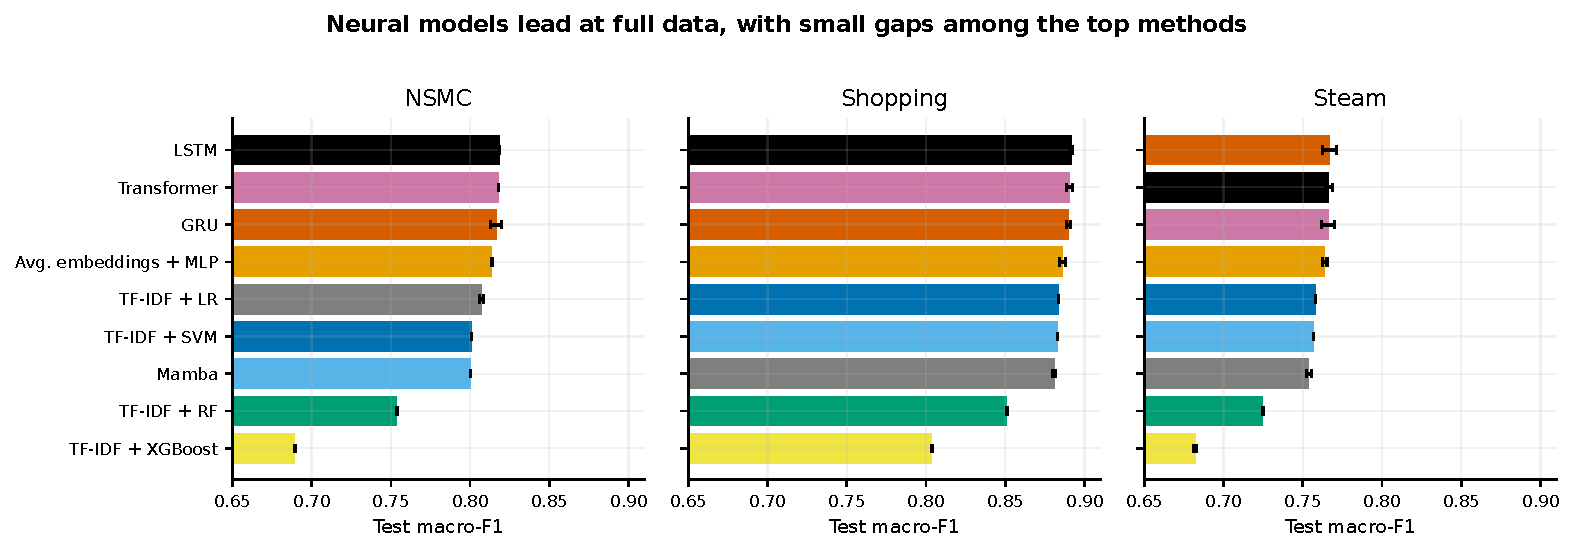
\includegraphics[width=0.86\textwidth]{full_data_comparison.pdf}
\end{frame}

\begin{frame}{Backup: NSMC confusion matrices}
  \centering
  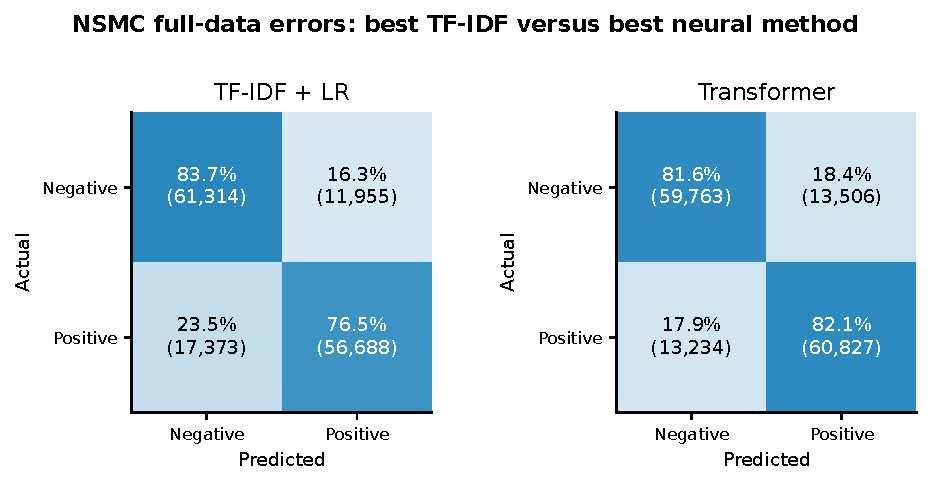
\includegraphics[width=0.7\textwidth]{confusion_comparison.pdf}
\end{frame}

\begin{frame}{Result audit and completeness}
  \centering
  \begin{tabular}{lrr}
    \toprule
    Phase & Completed & Expected\\
    \midrule
    Part 1 tuning & \Result{table_completeness_part1_tuning} & \Result{table_completeness_part1_tuning}\\
    Part 1 final & \Result{table_completeness_part1_final} & \Result{table_completeness_part1_final}\\
    Bonus tuning & \Result{table_completeness_bonus_tuning} & \Result{table_completeness_bonus_tuning}\\
    Bonus final & \Result{table_completeness_bonus_final} & \Result{table_completeness_bonus_final}\\
    \midrule
    Total & \Result{table_completeness_total} & \Result{table_completeness_total}\\
    \bottomrule
  \end{tabular}
  \vspace{4mm}

  \small Audit: complete with one declared derived-data correction. Atomic run values are unchanged.
\end{frame}

\begin{frame}{Backup: representation separation}
  \centering
  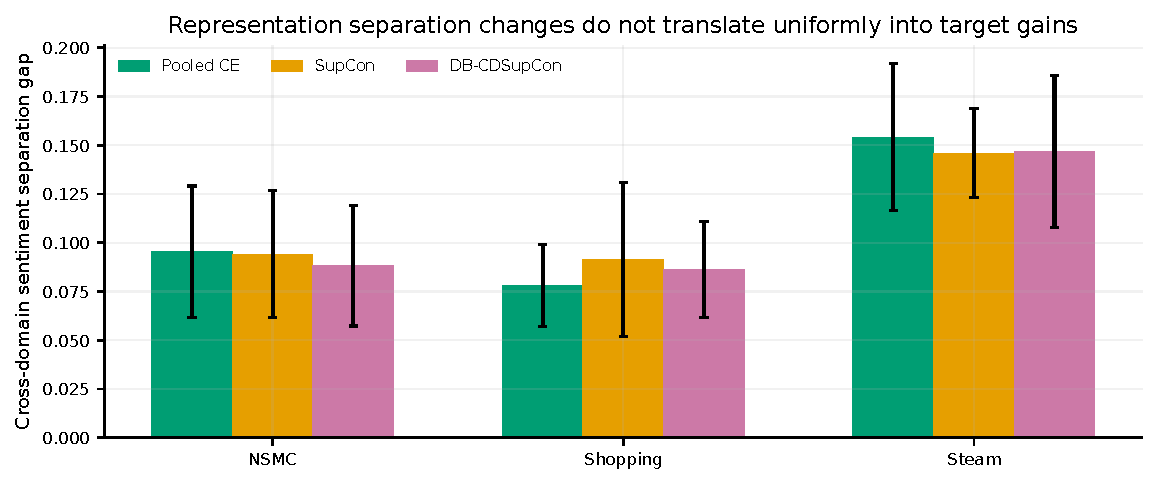
\includegraphics[width=0.78\textwidth]{bonus_representation.pdf}
\end{frame}

\begin{frame}{Tuning and frozen configurations}
  \begin{itemize}
    \item Part 1: ten predefined candidates per dataset-model pair at 8,000 labels
    \item Selector: validation macro-F1, latency, serialized size, configuration ID
    \item Bonus: four SupCon and eight DB-CDSupCon candidates per target
    \item Selector: target validation macro-F1, mean source validation macro-F1, fit time
    \item Test metrics absent from every tuning record
  \end{itemize}
\end{frame}

\begin{frame}{Backup: why no inference overhead from SupCon?}
  \[
    \text{tokens}\rightarrow \text{Transformer}\rightarrow h
    \begin{cases}
      \rightarrow \text{classifier} & \text{training and deployment}\\
      \rightarrow \text{projection}\rightarrow z & \text{training only}
    \end{cases}
  \]
  \begin{itemize}
    \item Projection head: \Result{bonus_projection_parameters} parameters
    \item Deployed Transformer and classifier: \Result{bonus_deployed_parameters} parameters
    \item SupCon and DB-CDSupCon change training loss, not deployed prediction
  \end{itemize}
\end{frame}

\end{document}
